\let\counterwithout\relax
\let\counterwithin\relax
\documentclass[final]{fhnwreport}       %[mode] = draft or final
\usepackage{color, colortbl}
\usepackage{rotating, rotfloat,ragged2e, hyphenat}

                                        %{class} = fhnwreport, article, 
                                        %          report, book, beamer, standalone
%%---Main Packages-----------------------------------------------------------------------
\usepackage[english, ngerman]{babel}	%Mul­tilin­gual sup­port for LaTeX
\usepackage[T1]{fontenc}				%Stan­dard pack­age for se­lect­ing font en­cod­ings
\usepackage[utf8]{inputenc}				%Ac­cept dif­fer­ent in­put en­cod­ings
\usepackage{lmodern}                    %The newer Font-Set
\usepackage{textcomp}					%LaTeX sup­port for the Text Com­pan­ion fonts
\usepackage{graphicx} 					%En­hanced sup­port for graph­ics
\usepackage{float}						%Im­proved in­ter­face for float­ing ob­jects
\usepackage{ifdraft}                    %Let you check if the doc is in draft mode

%%---Useful Packages---------------------------------------------------------------------
\usepackage[pdftex,dvipsnames]{xcolor}  %Driver-in­de­pen­dent color ex­ten­sions for LaTeX
\usepackage{csquotes}                   %Simpler quoting with \enquote{}
\usepackage{siunitx} 					%A com­pre­hen­sive (SI) units pack­age
\usepackage{listings}					%Type­set source code list­ings us­ing LaTeX
\usepackage[bottom]{footmisc}			%A range of foot­note op­tions
\usepackage{footnote}					%Im­prove on LaTeX's foot­note han­dling
\usepackage{verbatim}					%Reim­ple­men­ta­tion of and ex­ten­sions to LaTeX ver­ba­tim
\usepackage[textsize=footnotesize]{todonotes} %Mark­ing things to do in a LaTeX doc­u­ment

%%---Tikz Packages-----------------------------------------------------------------------
\usepackage{standalone}
\usepackage{tikz}
\usepackage{circuitikz}
\usetikzlibrary{arrows}
\usetikzlibrary{calc}
\usetikzlibrary{intersections}

%%---Math Packages-----------------------------------------------------------------------
\usepackage{amsmath}					%AMS math­e­mat­i­cal fa­cil­i­ties for LaTeX
%\usepackage{amssymb}					%Type­set­ting symbols (AMS style)
%\usepackage{array}						%Ex­tend­ing the ar­ray and tab­u­lar en­vi­ron­ments
%\usepackage{amsthm}					%Type­set­ting the­o­rems (AMS style)

%%---Table Packages----------------------------------------------------------------------
\usepackage{tabularx}					%Tab­u­lars with ad­justable-width columns
%\usepackage{longtable}
\usepackage{multirow}					%Create tab­u­lar cells span­ning mul­ti­ple rows
\usepackage{multicol}					%In­ter­mix sin­gle and mul­ti­ple columns

%%---PDF / Figure Packages---------------------------------------------------------------
\usepackage{pdfpages}					%In­clude PDF doc­u­ments in LaTeX
\usepackage{pdflscape}					%Make land­scape pages dis­play as land­scape
\usepackage{subfig}					    %Fig­ures di­vided into sub­fig­ures

%%---Other Packages----------------------------------------------------------------------
%\usepackage{xargs}                     %De­fine com­mands with many op­tional ar­gu­ments

%%---Bibliography------------------------------------------------------------------------
\usepackage[style=ieee,urldate=comp,backend=biber, natbib=true]{biblatex}
\addbibresource{literature/bibliography.bib}

%%---Main Settings-----------------------------------------------------------------------
\graphicspath{{./graphics/}}			%Defines the graphicspath
%\geometry{twoside=false}				    %twoside=false disables the "bookstyle"
\setlength{\marginparwidth}{2cm}
\overfullrule=5em						%Creates a black rule if text goes over the margins => debugging


%%---User Definitions--------------------------------------------------------------------
%%Tabel-Definitions: (requires \usepackage{tabularx})
\newcolumntype{L}[1]{>{\raggedright\arraybackslash}p{#1}}    %column-width and alignment
\newcolumntype{C}[1]{>{\centering\arraybackslash}p{#1}}
\newcolumntype{R}[1]{>{\raggedleft\arraybackslash}p{#1}}

%%---Optional Package Settings-----------------------------------------------------------
%Listings-Settings: (requires \usepackage{listings}) => Example with Matlab Code
\lstset{language=Matlab,%
    basicstyle=\footnotesize\ttfamily,
    breaklines=false,%
    morekeywords={switch, case, otherwise},
    keywordstyle=\color{Blue},%
    tabsize=2,
    %morekeywords=[2]{1}, keywordstyle=[2]{\color{black}},
    identifierstyle=\color{Black},%
    stringstyle=\color{Purple},
    commentstyle=\color{Green},%
    showstringspaces=false,%without this there will be a symbol in the places where there is a space
    numbers=left,%
    numberstyle={\tiny \color{black}},% size of the numbers
    numbersep=9pt, % this defines how far the numbers are from the text
    %emph=[1]{word1, word2,...},emphstyle=[1]\color{red}
}							
			                %loads all packages, definitions and settings												
\title{Kleinwasserkraftwerk}          	%Project Title
\author{Pflichtenheft}          		%Document Type => Technical Report, ...
\date{Windisch, 22.11.2018}             %Place and Date

\begin{document}

%%---TITLEPAGE---------------------------------------------------------------------------
\selectlanguage{ngerman}                %ngerman or english
\maketitle

\vspace*{-1cm}						    %compensates the space after the date line.
\vfill
\begin{figure}[H]
\centering

\includegraphics[width=\linewidth]{titelBild.jpg}
\end{figure}
\vfill

{
\renewcommand\arraystretch{2}
\begin{center}
\begin{tabular}{ >{\bf} l p{10cm} l }
Hochschule&Hochschule für Technik - FHNW\\
Studiengang&Elektro- und Informationstechnik\\
Autoren&Gruppe 4\\%Bachmann Lars \newline  Fischer Roni \newline Imhof Frank \newline Puschmann Pascal\\ 
Betreuer&Pascal Buchschacher\\
Auftraggeber&Felix Jenni\\
Version&1.0 %Normally not used!
\end{tabular}
\end{center}
}

\clearpage

%\selectlanguage{ngerman}				%ngerman or english
\thispagestyle{empty}
			
%%---TABLE OF CONTENTS-------------------------------------------------------------------
\pagenumbering{Roman}		
%\selectlanguage{ngerman}				%ngerman or english
\tableofcontents
\clearpage

%%---TEXT--------------------------------------------------------------------------------
\pagenumbering{arabic}
\section{Ãœbersicht} \label{sec:uebersicht}
\subsection{Ausgangslage}
Der Auftrag des Projekts 1 ist der Ersatz von Fossilen Ressourcen durch Elektrizität an einem ausgewählten Produkt. Das Team 4 hat sich das Ziel gesetzt, Lösungen zu finden, um die potentielle Energie des fallenden Abwassers in Hochhäusern und Wolkenkratzern in elektrische Energie umzuwandeln. Wird diese Energie zurück ins Gebäude gespeist, leistet unsere Lösung zwar keinen Ersatz von fossilen Ressourcen, aber einen Beitrag zur Reduktion des fossilen oder elektrischen Energieverbrauchs innerhalb von Gebäuden.
Durch die Recherchearbeit konnte das Team drei potentielle Lösungen finden, die nun in diesem technischen Teil des Pflichtenhefts weiter ausgearbeitet werden.
\renewcommand\arraystretch{1.5}
\definecolor{hr}{RGB}{255 200 200}
\definecolor{hgr}{RGB}{200 255 200}
\subsection{Ziele}
Folgende Ziele hat sich das Team 4 gesetzt:
\newcommand{\HY}{\hyphenpenalty = 25\exhyphenpenalty = 25}
\begin{table}[H]
\footnotesize
\begin{tabular}{>{\HY\RaggedRight}p{4.2cm} >{\HY\RaggedRight}p{3cm} >{\HY\RaggedRight}p{5cm} >{\HY\RaggedRight}p{1.8cm}}
\hline
\textbf{Zielkriterium}					&\textbf{Zielvariable}								&\textbf{Randbed.}												&\textbf{Gütekrit.}\\
\hline
\rowcolor{grau}
\multicolumn{4}{l}{\textbf{1. Elektrotechnik}}\\
1.1. Umwandlung der Energie					&Wirkungsgrad \%									&????															&>0.9\\
1.2. Funktion bei Ausfall					&Notumschalter									&Die Abwasserbeförderung funktioniert weiterhin.					&\\
1.3. Steuerun								&Anzeige											&Daten können ausgelesen werden. System kann abgeschaltet werden.	&\\
\rowcolor{grau}
\multicolumn{4}{l}{\textbf{2. Abwassertechnik}}\\
2.1. Steuerung								&Anzeige											&System kann überwacht und gesteuert werden.						&\\																&						&\\
2.2. Funktion bei Ausfall					&Bypass											&Die Abwasserbeförderung funktioniert weiterhin.					&\\
2.3. Platzbedarf								&Dimensionen	der zusätzlichen Infrastruktur[m3]	&kleiner als Platz im Modell										&\\
2.4. Instandhaltung							&Wartungsinterval [Jahre]								&Anzahl Jahre											&\\
\rowcolor{grau}
\multicolumn{4}{l}{\textbf{3. Finanzen}}\\
3.1. Materialkosten							&Kosten aller Bestandteile [CHF]					&liegen im Bereich einer Solaranlage mit vergleichbarer Leistung	&\\
3.2. Rendite									&Amortisationszeit	[Jahre]						&																&\\
\rowcolor{grau}
\multicolumn{4}{l}{\textbf{4. Sonstige}}\\
4.1. Lärmbelastung							&Lärmpegel [dB]									&																&\\
4.2. Integration								&Das System ist einfach zu integrieren.			&																&\\
\hline
\end{tabular}
\end{table}
\newpage
\subsection{Nicht-Ziele}
Da das Projekt 1 als Übung für die Abwicklung eines Projekts dient, werden sämtliche praktische Arbeiten wie Realisierung, Validierung und Projektabschluss nicht umgesetzt.\\
Auch der juristische Teil wird im Projekt 1 nicht beachtet.
Folgende Nicht-Ziele wurden definiert:
\begin{table}[H]
\begin{tabular}{ll}
\textbf{Nicht-Zielkriterium}				&\textbf{Nicht-Zielvariable}											\\
\hline
\rowcolor{grau}
\textbf{1. Planung}						&																	\\
										&Respektierung der Normen											\\
										&Machbarkeitsstudie													\\
\rowcolor{grau}
\textbf{2. Realisierung \& Kosten}		&																	\\
										&Einbau und Anschluss der Bestandteile\\
										&Testlauf															\\		
\hline
\end{tabular}
\end{table}

\section{Lösungskonzept} \label{sec:loesungskonzept}
\subsection{Problemstellung} \label{subsec:problemstellung}
Um eine erste Übersicht der möglichen Probleme des Lösungskonzepts zu erhalten, wurden folgende Punkte im Brainstormingverfahren zusammengetragen:
\begin{figure}[h]
	\centering
	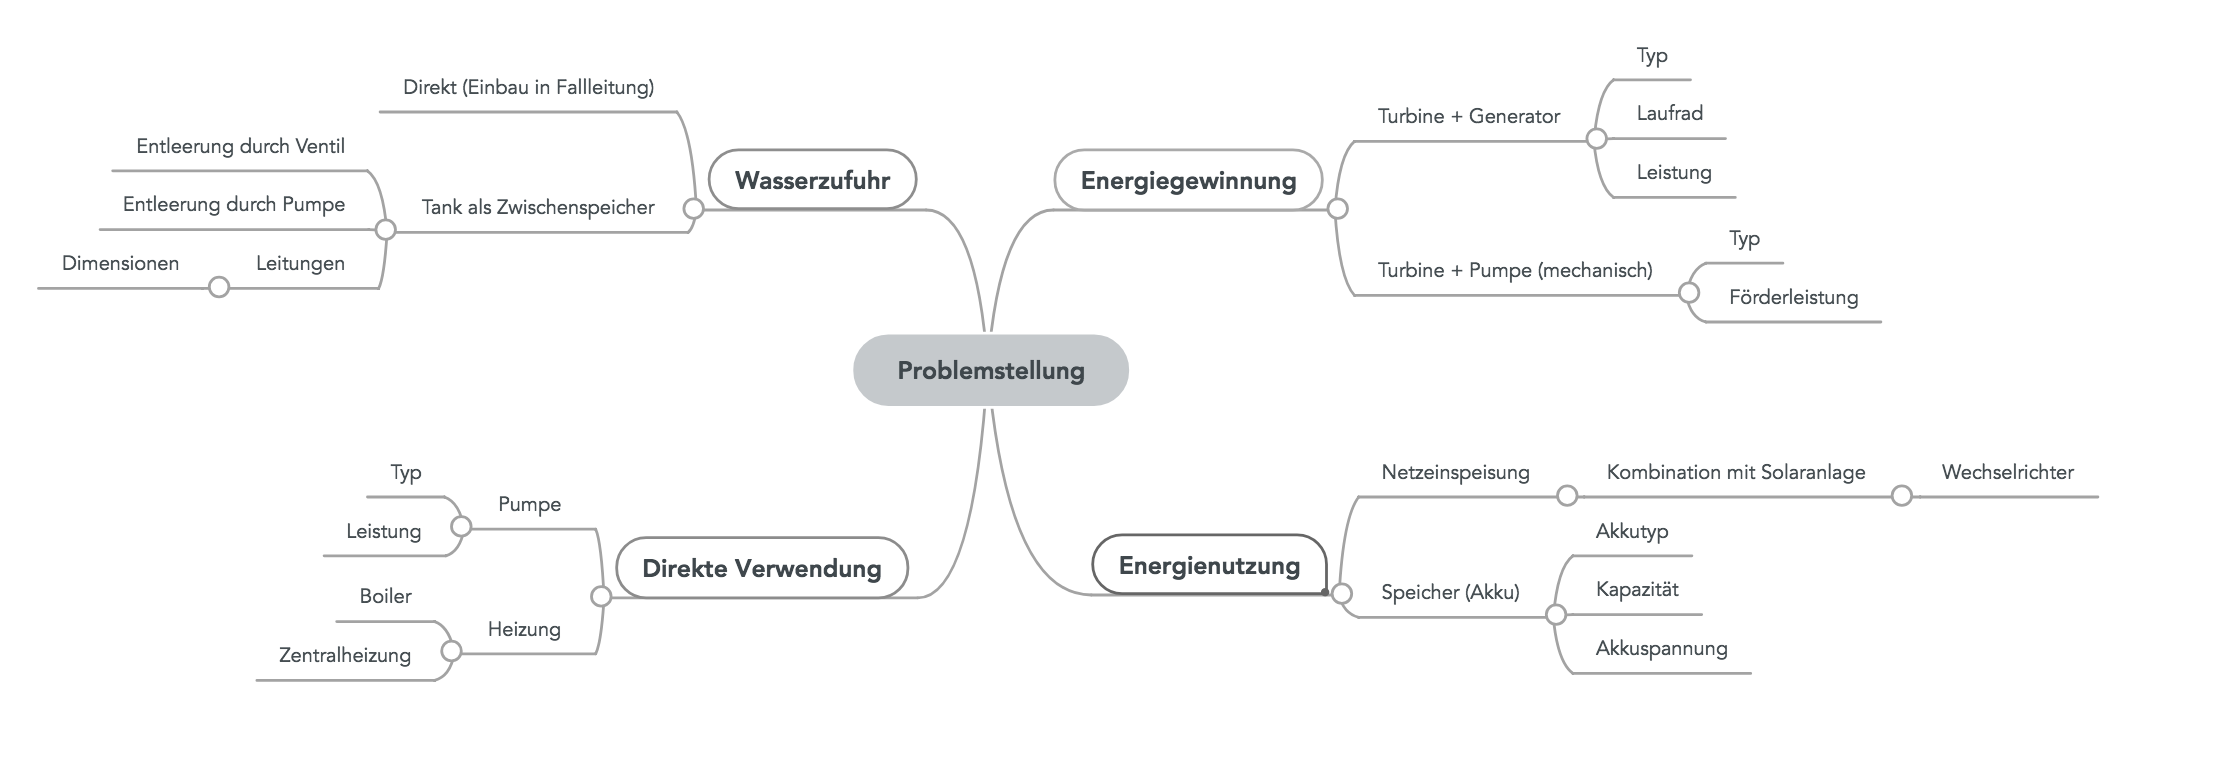
\includegraphics[width=0.9\linewidth]{Problemstellung.png}
	%\caption{}
	\label{fig:Figure}
\end{figure}
\subsection{Grobkonzept 1} \label{subsec:grobkonzept1}





\subsection{Grobkonzept 2} \label{subsec:grobkonzept2}
\begin{table}[H]
\footnotesize
\begin{tabular}{>{\HY\RaggedRight}p{3cm} >{\HY\RaggedRight}p{2.2cm} >{\HY\RaggedRight}p{4cm} >{\HY\RaggedRight}p{3.3cm} >{\HY\RaggedRight}p{1.2cm}}
\hline
	\textbf{Bestandteil}		&\textbf{Typ}			&\textbf{Funktion}									&\textbf{Specs}			&\textbf{Anz.}\\
\hline
\rowcolor{dgelb}
\multicolumn{5}{l}{\textbf{Stromerzeugung}}\\
	Turbine 					&Pelton 				&Umwandlung in Rotationsenergie						&							&1	\\
	Generator					&Gleichstrom 			&Umwandlung in elektrische Energie					&	 						&1	\\
\rowcolor{dblau}
\multicolumn{5}{l}{\textbf{Elektrotechnik}}\\
 	Wechselrichter				&						&Einspeisung ins Stromnetz							&							&1	\\
 	Zentrale Ventilsteuerung	&						&Öffnet/schliesst Ventile je nach Füllstand			&							&1	\\
\rowcolor{dpink}
\multicolumn{5}{l}{\textbf{Bedienung}}\\
 	Anzeige 					&LCD-Display			&zeigt Tankfüllstände und die Generatordaten an 	&							&1	\\
 	Warnsystem					&						&Warnt bei zu hochem Füllstand in einem der Tanks 	&							&1	\\
\rowcolor{dgruen}
\multicolumn{5}{l}{\textbf{Abwassertechnik}}\\
	Tanks 						& 						&Zwischenspeicher für Abwasser 						&4m3, trichterförmig		&5 	\\
	Ablassventil				&						&Entlässt das Abwasser aus dem Tank 				&							&5	\\
	Entlüftung					&						&Ermöglicht Luftaustausch, entlässt Gase			&							&5	\\
	Notüberlauf					&						&Verhindert, dass Tank zu voll wird					&							&5	\\
	Füllstandsensor				&Ultraschall			&Misst den Füllstand des Tanks						&Messbereich <20cm bis >3m	&5	\\
	Druckleitungen				&						&Machen hohe Wassersäulen möglich?					&Druckfestigkeit >40 bar	&5	\\
	Bypass für Turbine 			&Manuell				&Ermöglicht Wartung der Turbine 					&							&1	\\
	Bypass für Tanks 			&Manuell				&Ermöglicht Wartung und Reingung der Tanks 			&	 						&5	\\
	Einwegventile				&						&Verhindern Rückfluss 								&							&4	\\
\hline
\end{tabular}
\end{table}

Im Grobkonzept 2 soll die Energieausbeutung gesteigert werden, indem das Abwasser zuerst in Tanks gespeichert wird, die all ca. 13 Stockwerke eingebaut sind. In unserem Hochausmodell an der Park Avenue 432 in New York gibt es all ca. 13 Stockwerke ein Zwischenstockerk, wo der Einbau möglich wäre. Wenn der Füllstandsensor im Tank erkennt, dass er voll ist, wird ein Ventil geöffnet und das Wasser fliesst durch eine Druckleitung in den Keller, wo es eine Pelton-Turbine mit Generator antreibt. Die gewonnene Elektrische Energie wird über einen Wechselrichter dem Stromnetz zugeführt. 

Da das Abwasser das Rohr komplett ausfüllt, gibt es keinen Luftwiderstand, der es abbremst. So kann der Wirkungsgrad des Systems verbessert werden. Nur für eine Kurze zeit, bis das Rohr komplett mit Wasser gefüllt ist, tritt Luftwiderstand auf. Auf diese Art und Weise braucht man auch nur eine Turbine, die von mehreren Tanks gespeist werden kann. 

Die baulichen Massnahmen, die nötig sind, um dieses System zu installieren sind beträchtlich. Es müssen Tanks eingebaut werden, Druckleitungen zur Turbine verlegt werden, die im Keller installiert werden muss, und die bestehenden Abwasserleitungen anders verlegt werden, dass sie in die Tanks führen. Somit ist es eher für Neubauten geeignet als zur Nachrüstung.

\subsubsection{Wartung}
Um zu verhindern, dass es in den Tanks zu Ablagerungen kommt, ist der Boden der Tanks trichterförmig. So werden alle Ablageungen beim Öffnen des Ventils weggespült. Sollte es doch nötig sein, die Tanks zu Reinigen, gibt es ein Bypass mit dem das Abwasser an einem Tank vorbeigeführt werden kann. Er kann dass entleer und gereinigt oder repariert werden. Auch die Turbine hat einen Bypass, der Wartungsarbeiten ermöglicht.


\subsubsection{Sicherheitsmassnamen}
Jeder Tank ist mit einem Überlauf ausgestattet, der Verhindert, dass ein Tank zu voll wird wenn z.B. der Ablauf verstopft ist. Das überschüssige Abwasser wird dann in einem Rohr in die Fallleitung im darunterliegende Stockwerk geleitet. Von dort fliesst es dann in den nächsten Abwassertank. Der Füllstandssensor im Tank erkennt, wenn der Pegel zu hoch wird und sendet eine Warnung.
Falls aus irgendeinem Grund mehr als eines der Ventile gleichzeitig geöffnet würde, könnte es zu einem Rückstau kommen, bei dem Abwasser durch die Druckleitungen von dem höhergelegenen Tank in einen tieferen fliesst. Um dies zu verhindern,werden in den Druckleitungen Einwegventile eingebaut. Der höchstgelegene Tank benötigt kein solches Ventil. 


\textbf{Vorteile:} 									\newline
+	Kein Luftwiderstand (sobald Rohr gefüllt ist)	\newline
+	Nur eine Turbine nötig							\newline

\textbf{Nachteile:}									\newline
-	Braucht viel Platz 								\newline
-	Grössere Bauliche Massnahmen nötig				\newline
-	Verstopfungsgefahr 								\newline
-	Lange Leitungen brauchen länger bis komplett mit Wasser gefüllt, bis dann Luftwiderstand.



\subsection{Nutzwertanalyse} \label{subsec:nutzwertanlyse}
\renewcommand{\arraystretch}{1.5}
\newcommand{\vtcl}[1]{\rotatebox{90}{#1}}%\newcommand{\vtcl}[1]{\rotatebox{90}{\textbf{#1}}}
%\newcommand{\diagL}[1]{\diagbox{\hspace{#1}}{\hspace{#1}}}
Das Team konnte durch folgende Nutzwertanalyse bestimmen, welches Grobkonzept am ehesten in Fage kommt.
%\begin{table}[H]
%\small
%\begin{tabular}{l|llll|rr}
%&\vtcl{1.1. Wirkungsgrad}&\vtcl{1.2. Leistung}&\vtcl{1.3. Komplexität}&\vtcl{2.1. Platzbedarf}&\vtcl{Total}&\vtcl{Prozent}\\%\vtcl{2.1. Verstopfungsgefahr}&\vtcl{2.2. Platzbedarf}&\vtcl{2.3. Wartung}&\vtcl{Total}&\vtcl{Prozent}\\
%\hline
%1.1. Wirkungsgrad		&\cellcolor{black}	&0.5					&0.5					&0.5					&2.		&13\%\\
%1.2. Leistung			&0.5					&\cellcolor{black}	&1					&1					&4.5		&30\%\\
%1.3. Komplexität			&0.5					&0					&\cellcolor{black}	&0					&1.0		&6.5\%\\
%2.1. Verstopfungsgefahr	&1					&0					&1					&\cellcolor{black}	&0					&1					&3		&20\%\\
%2.1. Platzbedarf			&0.5					&0					&1					&\cellcolor{black}	&3.5		&24\%\\
%2.3. Wartung			&0.5					&0					&0.5					&0					&0					&\cellcolor{black}	&1.0		&6.5\%\\
%\hline
%\multicolumn{7}{c}{}&\textbf{15}&\textbf{100}\%\\
%\end{tabular}
%\end{table}
%\begin{scriptsize}
%Zeile-Kriterium ist wichtiger als Spalten-Kriterium 1\\
%Zeile-Kriterium ist gleich wichtig wie Spalten-Kriteriium 0.5\\
%Zeile-Kriterum ist weniger wichtig wie Spalternkriterium 0\\
%\end{scriptsize}
\newcolumntype{C}[1]{>{\centering}p{#1}}


\renewcommand\arraystretch{1.5}
\newcolumntype{R}[1]{>{\HY\RaggedLeft}p{#1}}
\newcolumntype{L}[1]{>{\HY\RaggedRight}p{#1}}
\renewcommand{\vtcl}[1]{\rotatebox{90}{\textbf{#1}}}
\begin{table}[H]
\caption{Nutzwertanalyse}\label{tab:nutzwertanalyse}
\small
\rotatebox{90}{
%|R{1.2cm}R{0.4cm}R{0.8cm} \scriptsize
%|R{1cm}R{0.2cm}R{0.5cm} \tiny
\begin{tabular}{lrR{0.8cm}|rrr|rrr|rrr|rrr|}%|R{1cm}R{0.5cm}R{0.8cm}
&&Max&\multicolumn{3}{c}{Grobkonzept 1}&\multicolumn{3}{c}{Grobkonzept 2}&\multicolumn{3}{c}{Grobkonzept 3}&\multicolumn{3}{c}{Grobkonzept 4}\\
\textbf{Zielkriterium}&\vtcl{Gewichtung}&\vtcl{Nutzwert}&\vtcl{Wert}&\vtcl{Erfüllungsgrad}&\vtcl{Nutzwert}&\vtcl{Wert}&\vtcl{Erfüllungsgrad}&\vtcl{Nutzwert}&\vtcl{Wert}&\vtcl{Erfüllungsgrad}&\vtcl{Nutzwert}&\vtcl{Wert}&\vtcl{Erfüllungsgrad}&\vtcl{Nutzwert}\\
\hline
&&&&&&&&&&&&&&\\
\rowcolor{hellgrau}
\multicolumn{3}{l|}{\textbf{Elektrotechnik}}&\multicolumn{3}{r|}{}&\multicolumn{3}{r|}{}&\multicolumn{3}{r|}{}&\multicolumn{3}{r|}{}\\
%										%G1 Wert		%G1 Erf.		G1 Nutz			%G2 Wert		%G2 Erf.		G2 Nutz			%G3 Wert		%G3 Erf.		G2 Nutz			%G4 Wert		%G4 Erf.		G4 Nutz
1.1. Wirkungsgrad	&25\%		&1.25	&32\%		&1			&0.25			&67.2\%		&3			&0.75			&64.1\%		&3			&0.75			&80\%		&4			&1.00\\
1.2. Leistung		&30\%		&1.50	&21.5kWh		&1			&0.33			&44.6kWh		&2			&0.66			&42.6kWh		&2			&0.66			&53.1kWh		&4			&1.20\\
%&&&&&&&&&&&&&&\\
\rowcolor{hellgrau}
\multicolumn{3}{l|}{\textbf{Abwassertechnik}}&\multicolumn{3}{r|}{}&\multicolumn{3}{r|}{}&\multicolumn{3}{r|}{}&\multicolumn{3}{r|}{}\\
%Verstopfungssicherheit&20\%		&1.000	&mässig		&2			&0.40			&mässig		&2			&0.4	0			&mässig		&2			&0.40			&mittel		&3			&0.60\\
2.1. Platzsparung	&25\%		&1.00	&erhöht		&4			&1.00			&mässig		&2			&0.50			&mässig		&2			&0.50			&erhöht		&4			&1.00\\
%Wartung				&6.5\%		&0.325	&5			&2			&0.26			&3			&2			&0.26			&1			&4			&0.20			&1			&4			&0.20\\
\rowcolor{hellgrau}
\multicolumn{3}{l|}{\textbf{Allgemein}}&\multicolumn{3}{r|}{}&\multicolumn{3}{r|}{}&\multicolumn{3}{r|}{}&\multicolumn{3}{r|}{}\\
3.1. Schlichtheit	&20\%		&1.00	&8			&4			&0.8	0			&14			&3			&0.60			&15			&3			&0.60			&10			&4			&0.80\\
&&&&&&&&&&&&&&\\
\hline
Summe				&100.0\%		&5.000	&			&			&2.38			&			&			&2.51			&			&			&2.51			&			&			&4.00\\
Erfüllungsgrad [\%]	&&100.0				&			&			&48				&			&			&50				&			&			&50				&			&			&80\\
\multicolumn{3}{l}{\textbf{Rangfolge}}&\multicolumn{3}{r|}{\textbf{3}}&\multicolumn{3}{r|}{\textbf{2}}&\multicolumn{3}{r|}{\textbf{2}}&\multicolumn{3}{r|}{\textbf{1}}\\
\multicolumn{15}{l}{\textbf{}}\\
\multicolumn{15}{l}{\textbf{}}\\
\end{tabular}
}
\rotatebox{90}{
\scriptsize
\begin{tabular}{lC{1.2cm}C{1.2cm}C{1.2cm}C{1.2cm}C{1.2cm}l}
\multicolumn{7}{c}{\textbf{Erfüllungsgrad}}\\
\hline
&min.&&mittel&&max.&\\
&\textbf{1}&\textbf{2}&\textbf{3}&\textbf{4}&\textbf{5}&Messgrösse\\
\hline
1.1. Wirkungsgrad				&<50&51-60&61-70&71-80&>81&\%\\
1.2. Leistung					&<40&40-44&45-50&51-54&>55&kWh\\
%2.1. Verstopfungssicherheit		&gering&mässig&mittel&erhöht&hoch&a)\\
2.1. Platzsparung				&gering&mässig&mittel&erhöht&gross&Schätzung m\textsuperscript{3}\\
%2.3. Wartung						&52-13&12-6&5-2&1&0&b)\\
3.1. Schlichtheit				&>20&20-16&15-11&10-6&1-5&Anz. versch. Teile\\
\end{tabular}
}
\end{table}






\section{Auswertung} \label{sec:auswertung}

\subsection{Modell} \label{subsec:modell}

Für die Berechnung der potentiellen Energie benützen wir das Modell Park Avenue 432, eines der höchsten reinen Wohnhochhäusern auf der Welt. Die stolze Höhe und der über das ganze Gebäude gleichbleibende quadratische Grundriss sind ideal für unsere Berechnungen. Für die Wassermengenberechnung stützen wir uns auf die Angaben des durchschnittlichen Wasserverbrauch in Amerika pro Person und Tag: 314\si{L}. \cite{waterUsAmerica}

\begin{figure} [H]
	\centering
	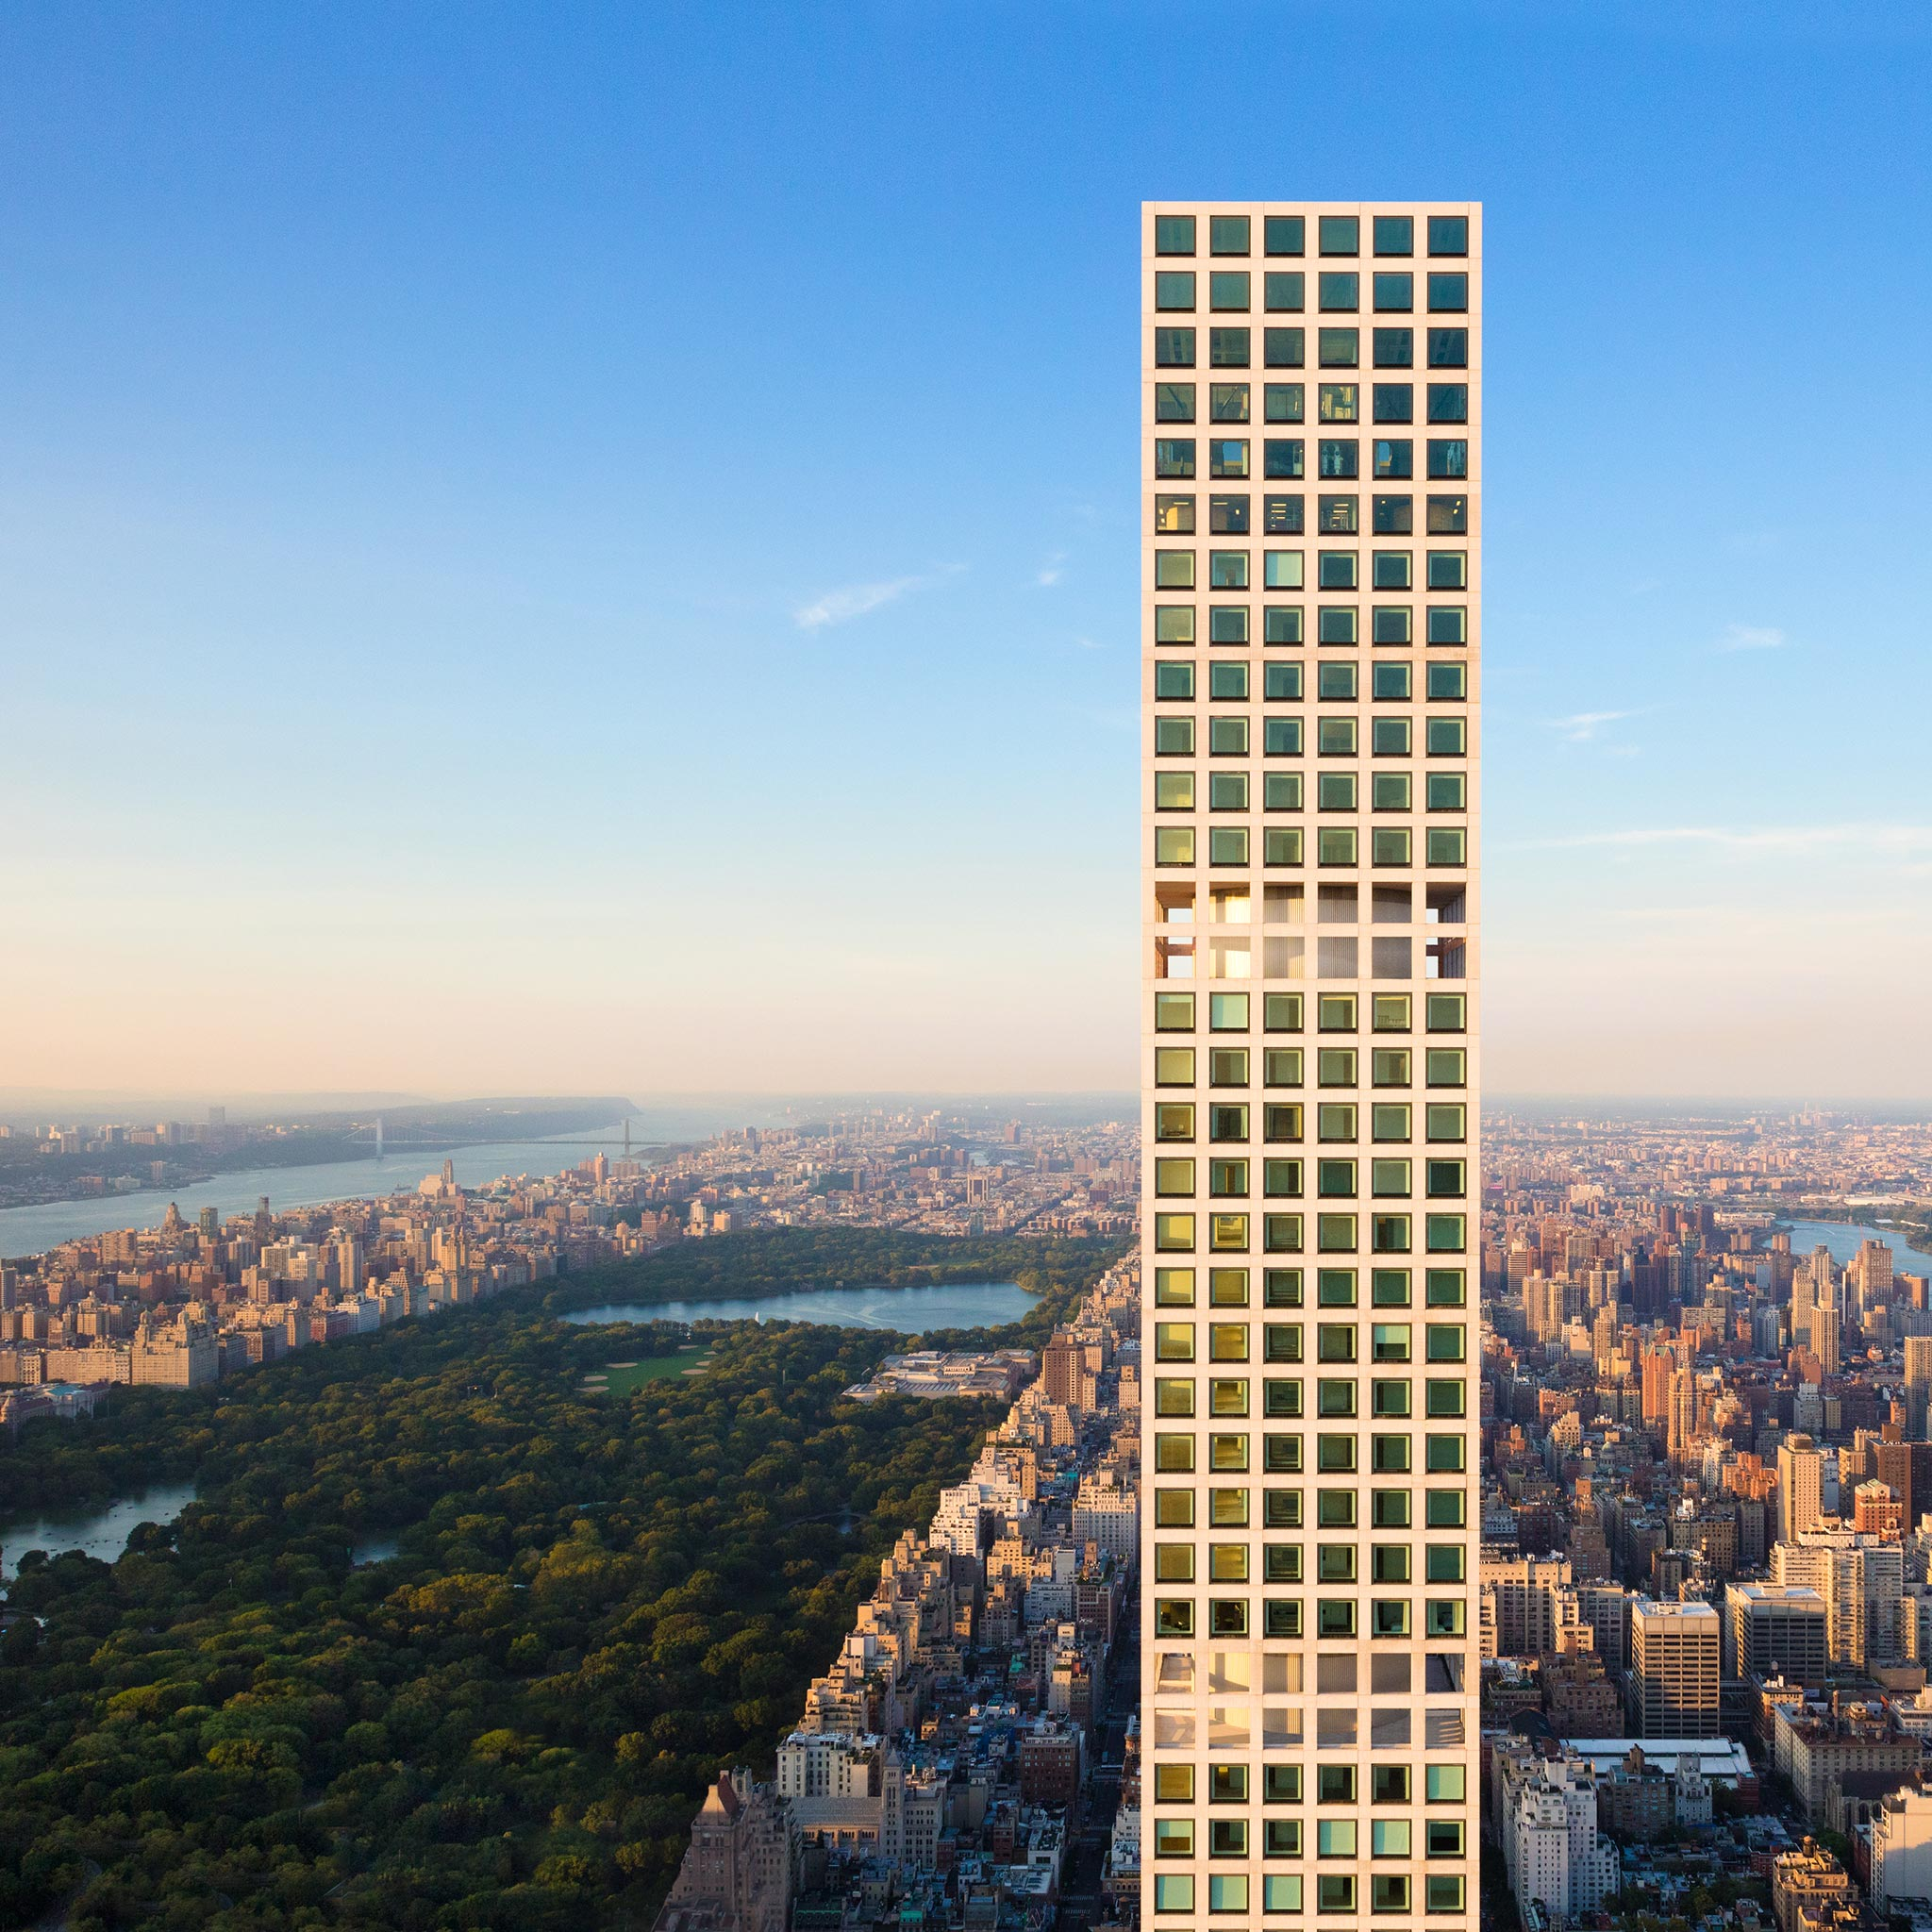
\includegraphics[width=12cm]{parkAvenue.jpg}
	\caption{Park Avenue 432 \cite{432_Park_Avenue}}
	\label{fig:Park_Avenue_432}
\end{figure}

\begin{table}[H]
\centering
\begin{tabular}{ll}
Name:				&Park Avenue 432\\
Höhe: 				&426m\\          
Etagen:				&84 Obergeschosse, 1 Erdgeschosse, 3 Untergeschosse\\
Etagenhöhe:			&4.72m\\
Hoechste Etage:		&392.1m\\
Wohnungen:			&146\\
Speziell:			&alle 12 Etagen 2 Etagen leer\\           
\end{tabular}
\end{table}

\newpage


\subsection{Energieberechnung} \label{subsec:energieberechnung}

Die Endgeschwindigkeit des Wassers kann mit folgender Formel berechnet werden:
\begin{center}
\(v = \sqrt{2 \cdot g \cdot h} \)
\end{center}

Die Einheit der Geschwindigkeit \(v\) ist \si{m/s}, das Schwerefeld \(g\) auf der Erde besitzt den Wert 9.81~\si{N/kg}, und die Höhe \(h\) hat die Einheit \si{m}.

\bigskip

Die Energie, die gewonnen werden kann, wird mit folgender Formel berrechnet:

\begin{center}
\(E =\frac 12\ \cdot m \cdot v^2\)
\end{center}

Die Energie \(E\) hat die Einheit \si{J}, die Einheit der Geschwindigkeit \(v\) ist \si{m/s}, und die Masse \(m\) hat die Einheit \si{kg}

\bigskip

Um die Leistung zu erhalten, muss die Masse pro Zeit(1s) einberechnet werden. Die Masse wird mit der Dichte und dem Volumenstrom ersetzt.

\begin{center}
\(P =\frac 12\ \cdot \varphi \cdot Q \cdot v^2\)
\end{center}

Die Leistung \(P\) hat die Einheit \si{W}, der Volumentstrom \(Q\) die Einheit \si{m^3/s}, die Dichte \(\varphi\) \si{kg/m^3} und die Geschwindigkeit \(v\) \si{m/s}.

\newpage

Mit diesen Mathematischen Grundlagen kann nun die Energie an unserem Modellhochhaus für beide Grobkonzepte berechnet werden. Für die Berchnungen wird angenommen das pro Wohnung 2.5 Personen leben und sie einen Durchschnittverbrauch pro Tag von 314\si{L} haben.

Bei 146 Wohnungen und 74 Nutzbaren Etagen leben 5 Personen pro Etage. Es wird somit 1570\si{L} pro Etage pro Tag verbraucht.

\bigskip

\paragraph{Grobkonzept 1} 



\paragraph{Grobkonzept 2}

Mit dem Grobkonzept 1 kommt man total auf ********. Mit dem Grobkonzept 2 kommt man total auf *******. Die Berechnungen sind im Anhang unter  ersichtlich \ref{subsec:grobkonzept1} \nameref{subsec:grobkonzept1} und \ref{subsec:grobkonzept2} \nameref{subsec:grobkonzept2} ersichtlich




\subsection{Kostenberechnung} \label{subsec:kostenberechnung}
\section{Kosten}

\section{Wirtschaftlichkeit} \label{sec:wirtschaftlichkeit}
In diesem Abschnitt berechnen wir anhand grober Schätzungen die Wirtschaftlichkeit unseres Systems. 
Als Indikator für die Wirtschaftlichkeit wird die Amortisationszeit verwendet.
\subsection{Annahmen}
Für die vereinfachung der Amortisationsrechnung wurden folgende Annahmen getroffen:\\
\begin{itemize}  
\item Das Hochhaus wird neu gebaut, deshalb entstehen keine Umbaukosten.
\item Als Investitionskosten zählen wir die Einbaukosten der zusätzlichen Infrastruktur, die Materialkosten und die Entwicklungskosten.
\item Pro Jahr entsteht ein Service- und Reperaturaufwand in der Höhe von schätzungsweise 1'000 CHF.
\item Die Einbaukosten der zusätzlichen Infrastruktur betragen etwa 10'000 CHF.
\item Das System hat eine Lebensdauer von 50 Jahren.
\end{itemize}

\renewcommand\arraystretch{1.2}
\newcolumntype{Z}[1]{>{\HY\RaggedLeft\bfseries}p{#1}}
\subsection{Kosten}
\begin{table}[H]
\small
\begin{tabular}{L{4cm}R{1.5cm}rR{2cm}Z{2cm}}
%\multicolumn{4}{l}{\textbf{Investitionskosten}}\\
\hline
\textbf{Kostenkategorie}&\textbf{Anzahl}&\textbf{Preis[CHF]/Element}&\textbf{Preis[CHF]}&\\
\hline
\rowcolor{hellgrau}
\multicolumn{4}{l}{\textbf{Einbaukosten}}&10'000\T\\
Einbau zus. Infrastruktur&1&10'000&10'000&\B\\
\rowcolor{hellgrau}
\multicolumn{4}{l}{\textbf{Materialkosten}}&88'160\T\\
\multicolumn{4}{l}{\textit{Mechanik}}&\normalfont{69'000}\\
Rohrkette 60.08m&5&10'000&50'000&\\
Rohrkette 80.24m&1&13'000&13'000&\\
Zahnradsystem&6&1000&6'000&\\
\multicolumn{4}{l}{\textit{Elektrotechnik}}&\normalfont{11'760}\T\\
Generator&6&110&660&\\
Gleichrichter&6&300&1'800&\\
Wechselrichter&1&3'401&3'401&\\
Kontrollsystem&1&5900&5900&\\
\multicolumn{4}{l}{\textit{Abwassertechnik}}&\normalfont{7'400}\T\\
Umleitventil&74&100&7'400&\B\\
\rowcolor{hellgrau}
\multicolumn{4}{l}{\textbf{Entwicklungskosten}}&48'000\T\\
Software&1&48'000&48'000\B\\
\hline
%\rowcolor{grau}
\multicolumn{3}{l}{\textbf{Gesamt}}&&146'160\T\\
&&&\\
&&&\\
\end{tabular}
\caption{Kostentabelle}\label{tab:kostentabelle}
\end{table}
\newpage
\subsection{Amortisationszeit}
Mit der Formel $A = \tfrac{K}{R}$ wird nun die Amortisationszeit (A) berechnet, wobei K die einmaligen Investitionskosten sind, die man aus der Tabelle \ref{tab:kostentabelle} entnehmen kann. R ist der jährliche Rückfluss, also in unserem Fall der Ertrag aus dem Stromgewinn abzüglich des Service- und Reperaturaufwands.\\

\bigskip
K = 146'160 CHF

\bigskip
R = 365$\tfrac{T}{J}\cdot$10.62$\tfrac{CHF}{T}$ - 1'000$\tfrac{CHF}{J}$ = 2'876$\tfrac{CHF}{J}$

\bigskip
$A = \tfrac{146'160CHF}{2'876 \tfrac{CHF}{J}} =$ 50.82$J$
\section{Projektvereinbarung}
\textbf{Auftraggeber}
Jenni, Prof. Dr. Felix
\bigskip
\hrule
Ort, Datum
\bigskip
\hrule
Ort, Datum


%%---BIBLIOGRAPHY------------------------------------------------------------------------

{\sloppypar
\selectlanguage{english}	
\setlength{\bibitemsep}{\baselineskip}
\printbibliography[heading=bibintoc]
\label{sec:lit}
}

%%---NOTES for DEBUG---------------------------------------------------------------------
\ifdraft{%Do this only if mode=draft
%%requires \usepackage{todonotes})
\newpage
\listoftodos[\section{Todo-Notes}]
\clearpage
}
{%Do this only if mode=final
}
\end{document}
